%%% Класс документа
\documentclass[a4paper,14pt]{article}

%%% Работа с русским языком
\usepackage{cmap}					% поиск в PDF
\usepackage[warn]{mathtext}
\usepackage[T2A]{fontenc}			% кодировка
\usepackage[utf8]{inputenc}			% кодировка исходного текста
\usepackage[english,russian]{babel}	% локализация и переносы
\usepackage{mathtext} 				% русские буквы в формулах
\usepackage{csvsimple}              % for tabular from csv loading
\usepackage{indentfirst}            % indent after sections
%\usepackage{minipage}

%%% Дополнительная работа с математикой
\usepackage{amsmath,amsfonts,amssymb,amsthm,mathtools} % AMS
\usepackage{icomma} % "Умная" запятая: $0,2$ --- число, $0, 2$ --- перечисление

%%% Номера формул
%\mathtoolsset{showonlyrefs=true} % Показывать номера только у тех формул, на которые есть \eqref{} в тексте.
%\usepackage{leqno} % Немуреация формул слева

%%% Шрифты
\usepackage{euscript}	 % Шрифт Евклид
\usepackage{mathrsfs} % Красивый матшрифт

%%% Свои команды
\DeclareMathOperator{\sgn}{\mathop{sgn}}

%%% Перенос знаков в формулах (по Львовскому)
\newcommand*{\hm}[1]{#1\nobreak\discretionary{}
{\hbox{$\mathsurround=0pt #1$}}{}}

%%% Работа с картинками
\usepackage{graphicx}  % Для вставки рисунков
\graphicspath{{images/}{images2/}}  % папки с картинками
\setlength\fboxsep{3pt} % Отступ рамки \fbox{} от рисунка
\setlength\fboxrule{1pt} % Толщина линий рамки \fbox{}
\usepackage{wrapfig} % Обтекание рисунков и таблиц текстом

%%% Работа с таблицами
\usepackage{array,tabularx,tabulary,booktabs} % Дополнительная работа с таблицами
\usepackage{longtable}  % Длинные таблицы
\usepackage{multirow} % Слияние строк в таблице

%%% Теоремы
\theoremstyle{plain} % Это стиль по умолчанию, его можно не переопределять.
%\newtheorem{theorem}{Теорема}[section]
%\newtheorem{proposition}[theorem]{Утверждение}
 
%\theoremstyle{definition} % "Определение"
%\newtheorem{corollary}{Следствие}[theorem]
%\newtheorem{problem}{Задача}[section]
 
%\theoremstyle{remark} % "Примечание"
%\newtheorem*{nonum}{Решение}

%%% Программирование
\usepackage{etoolbox} % логические операторы

%%% Страница
\usepackage{extsizes} % Возможность сделать 14-й шрифт
\usepackage{geometry} % Простой способ задавать поля
	\geometry{top=25mm}
	\geometry{bottom=35mm}
	\geometry{left=35mm}
	\geometry{right=20mm}
	
%%% Колонтитулы
%\usepackage{fancyhdr}
 	%\pagestyle{fancy}
 	%\renewcommand{\headrulewidth}{0mm}  % Толщина линейки, отчеркивающей верхний колонтитул
 	%\lfoot{Нижний левый}
 	%\rfoot{Нижний правый}
 	%\rhead{Верхний правый}
 	%\chead{Верхний в центре}
 	%\lhead{Верхний левый}
 	% \cfoot{Нижний в центре} % По умолчанию здесь номер страницы
 	
%%% Интерлиньяж
%\usepackage{setspace}
%\onehalfspacing % Интерлиньяж 1.5
%\doublespacing % Интерлиньяж 2
%\singlespacing % Интерлиньяж 1

%%% Гиперссылки
\usepackage{hyperref}
\usepackage[usenames,dvipsnames,svgnames,table,rgb]{xcolor}
\hypersetup{				% Гиперссылки
    unicode=true,           % русские буквы в раздела PDF
    pdftitle={Заголовок},   % Заголовок
    pdfauthor={Автор},      % Автор
    pdfsubject={Тема},      % Тема
    pdfcreator={Создатель}, % Создатель
    pdfproducer={Производитель}, % Производитель
    pdfkeywords={keyword1} {key2} {key3}, % Ключевые слова
    colorlinks=true,       	% false: ссылки в рамках; true: цветные ссылки
    linkcolor=red,          % внутренние ссылки
    citecolor=green,        % на библиографию
    filecolor=magenta,      % на файлы
    urlcolor=cyan           % на URL
}

%%% Другие пакеты
\usepackage{lastpage} % Узнать, сколько всего страниц в документе.
\usepackage{soul} % Модификаторы начертания
\usepackage{csquotes} % Еще инструменты для ссылок
%\usepackage[style=authoryear,maxcitenames=2,backend=biber,sorting=nty]{biblatex}
\usepackage{multicol} % Несколько колонок
\usepackage{multirow} % Несколько строк

%%% Шрифты
%\renewcommand{\familydefault}{\sfdefault} % Начертание шрифта


%%% Работа с библиографией
%\usepackage{cite} % Работа с библиографией
%\usepackage[superscript]{cite} % Ссылки в верхних индексах
%\usepackage[nocompress]{cite} % 
%\usepackage{csquotes} % Еще инструменты для ссылок


%%% Tikz
\usepackage{tikz} % Работа с графикой
\usepackage{pgfplots} % Работа с pgf
\usepackage{pgfplotstable}
\usepackage{upgreek}

%%% Дополнительные пакеты для tikz
%\usepgfplotslibrary{dateplot} % Возможность подписания дат
\pgfplotsset{compat=1.5}

\begin{document}
    % \newcommand{\HRule}{\rule{\linewidth}{0.7mm}} % Defines a new command for the horizontal lines, change thickness here
	
	\begin{center}
		\large\textbf{Московский Физико-Технический Институт}\\ % Name of your university/college
		\large\textbf{(государственный университет)}
	
		\vfill
		
		\Large Лабораторная работа по курсу общей физики № *labnum*\\[0.5cm] % Preambule of your document title
		
		
		\HRule
		\\[0.4cm]
		{ \huge \bfseries *name of your labwork*}% Title of your document
		\\[0.4cm] 
		\HRule
		\\[0.5cm]
		
		\ \\
	\textbf{\large Автор:} \\	
	\large *your name* *groupname*\\ % Your name and something more, your group num for example
		\vfill
		\hspace*{-0.8 cm}
\includegraphics[width=100 pt]{frkt_logo}\\ % logo of your  company/university/college
		\large Долгопрудный, 2021 % location and year
	\end{center}

\newpage
\setcounter{page}{2}
\fancyfoot[c]{\thepage}
\fancyhead[L] {Работа № *labnum*} % some information in page header
\fancyhead[R]{}

    Измерим параметры магнитных шариков: $m_1 = 820$ г, $m_2 = 815$ г, $d = 5,9$ мм.\\
    Величину магнитного момента двух одинаковых шариков можно расчитать, зная их массу и определив
    максимальное расстояние $r_{max}$, на котором они удерживают друг друга.

    \begin{equation*}
        P_m = \sqrt{\frac{4 \pi mg r_{max}^4}{6 \mu_0}}
    \end{equation*}

    Перепишем выражение с учетом $\mu_0 = 4 \pi \cdot 10^{-7}$

    \begin{equation*}
        P_m = \sqrt{\frac{mg r_{max}^4}{6} \cdot 10^7}
    \end{equation*}

    В процессе эксперемента получено $r_{max} = 23$ мм.

    \begin{center}
        \fbox{$P_m = 61,84 ~ \text{А} \cdot \text{м}^2$}
    \end{center}

    Горизонтальную составляющую магнитного поля Земли можно найти, используя период крутильных колебаний.

    \begin{equation*}
        T = 2 \pi \sqrt{\frac{J_n}{P_{mn} B_{||}}}
    \end{equation*}
    где $J_n$ -- момент инерции стрелки из $n$ шариков, $P_{mn} = P_m \cdot n$ -- магнитный момент стрелки.
    Момент инерции стрелки приближенно можно считать
    \begin{equation*}
        J_n \approx \frac{1}{3} n^3 m R^2
    \end{equation*} 
    тогда
    \begin{equation*}
        T = 2 \pi \sqrt{\frac{m R^2}{3 P_m B_{||}}} n
    \end{equation*}

    Снимем зависимость и построим график $T(n)$, тогда угловой коэффициент наклона будет равен $k = 2 \pi \sqrt{\frac{m R^2}{3 P_m B_{||}}}$.
    От сюда найдем горизонтальную составляющую магнитного поля Земли: $B_{||} = \frac{m R^2}{3 P_m k^2}$.

    \begin{table}[h!]
        \begin{center}
            \begin{tabular}{|c|c|c|c|c|c|}
                \hline
                $n$ & 11   & 10   & 9   & 8    & 7    \\ \hline
                $T$ & 2,86 & 2,67 & 2,4 & 2,23 & 1,95 \\ \hline
            \end{tabular}
        \end{center}
    \end{table}

    % вставить график

    \begin{center}
        \fbox{$B_{||} = $ мкТл}
    \end{center}

    Измерить вертикальную составляющую магнитного поля Земли можно с помощью той же установки, используя уравнение моментов.

    \begin{equation*}
        m g r_{\text{гр}} = n P_m B_{\perp}
    \end{equation*}

    \begin{center}
        \fbox{$B_{\perp} = 49,9 $ мкТл}
    \end{center}

    Найдем польный модуль магнитного поля Земли на текущей широте.

    \begin{equation*}
        B_0 = \sqrt{B_{||}^2 + B_{\perp}^2} = ~ \text{мкТл}
    \end{equation*}

    Исследуем индукцию соленоида. Параметры шайбы: $d = 9$ мм, $h = 4$ мм.

    \begin{table}[h!]
        \begin{center}
            \begin{tabular}{|c|c|c|c|c|c|c|c|c|}
                \hline
                $n$      & 1   & 2   & 3   & 4   & 5   & 6   & 7   & 8   \\ \hline
                $B$, мТл & 232 & 314 & 349 & 355 & 362 & 363 & 364 & 369 \\ \hline
            \end{tabular}
        \end{center}
    \end{table}

    \begin{figure}[h!]
        \centering
        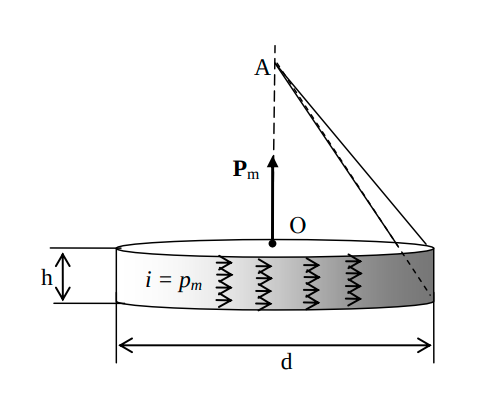
\includegraphics[scale = 0.5]{индукция соленоида.png}
        \caption{}
    \end{figure}

    Магнитное поле в произвольной точке $A$ на оси соленоида расчитывается по формуле

    \begin{equation*}
        B_A = \frac{\mu_0}{4 \pi} 2 \pi i (\cos \alpha - \cos \beta)
    \end{equation*}

    Для точки $O$ на торце соленоида $\cos \beta = 0$, так что для соленоида высотой $h$, радиусом $R$, и магнитным моментом
    $P_m$ поле на торце расчитывается по формуле

    \begin{equation*}
        B(h) = \frac{\mu_0}{2} P_m \frac{h}{\sqrt{R^2 + h^2}}
    \end{equation*}

    Проведем небольшое исследование функции $B(h)$.

    \begin{equation*}
        \lim_{h \rightarrow \infty} \frac{\mu_0}{2} P_m \frac{h}{\sqrt{R^2 + h^2}} = \frac{\mu_0}{2} P_m
    \end{equation*}

    Таким образом, график функции $B(h)$ должен иметь горизонтальную асимптоту $B_0 = \frac{\mu_0}{2} P_m$, что мы и можем
    наблюдать на практике.

    \begin{figure}[h!]
        \centering
        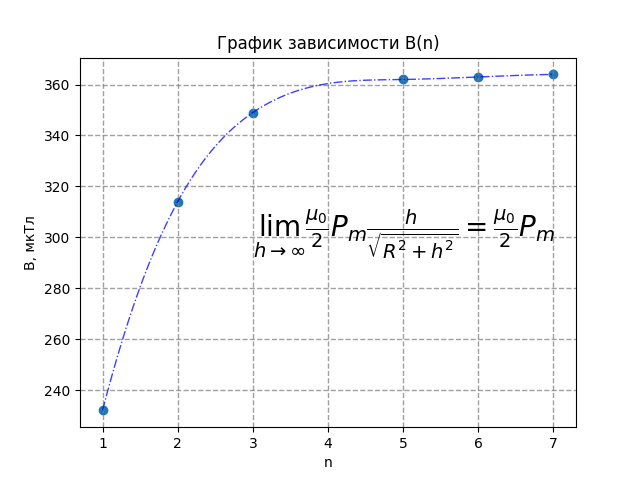
\includegraphics[scale = 1]{solenoid.png}
        \caption{}
    \end{figure}

\end{document}